\section{Maintenance}

Overview text required.





\subsection{Firmware}

The entire AXIOM Beta firmware is stored on a Micro SD card. This means that the camera's operating system can be swapped out easily and that external recovery of the camera entire software, in case anything went wrong eg. during flashing, is always possible.\\ 

It also means that experimental features can easily be tried and tested simply by popping in a different card into the camera. 





\subsubsection{Firmware Backup}

The entire camera firmware is stored on a Micro SD card plugged into the Microzed. To back-up the entire firmware we plug in the Micro SD card into a Linux PC and do the following:

1. Find out which device the micro SD card is: 

\consoleCommand{    cat /proc/partitions
    mount}

... should give you a list of all connected devices. Lets assume in our case that the card is /dev/sdc.\\


2. Make sure the card is unmounted (all 3 partitions): 

\consoleCommand{    umount /dev/sdc1
    umount /dev/sdc2
    umount /dev/sdc3t}
    
    
3. clone the entire card to a file: 

\consoleCommand{ddrescue /dev/sdc sdimage.img sdimage.log}

Here is a guide that covers doing the same on Mac and Windows: \href{http://raspberrypi.stackexchange.com/questions/311/how-do-i-backup-my-raspberry-pi}{http://raspberrypi.stackexchange.com/questions/311/how-do-i-backup-my-raspberry-pi}






\subsubsection{Firmware Restore}

Again you need to know the device path of your sd card, then (assuming in our case its /dev/sdb) run:

\consoleCommand{sudo dd if=sdimage.img of=/dev/sdb bs=4M}






\subsection{Image Sensor cleaning}

We are using the green sensor cleaning swabs:

\begin{center}

\includegraphics[height=5cm]{images/Green_Swabs_200X200_B}
\end{center}

It comes with two cleaning solutions: one for dust and one for any oil based residues (finger prints, etc.)\\

On this page we try to collect typical sensor contamination images, guides how to spot and get rid of them.\\

The best lighting conditions to spot contamination seems to be mid grey, you can take off or slightly turn the lens to make sure the contamination is not on any lens glass element.\\

Vertical streaks:\\

\begin{center}
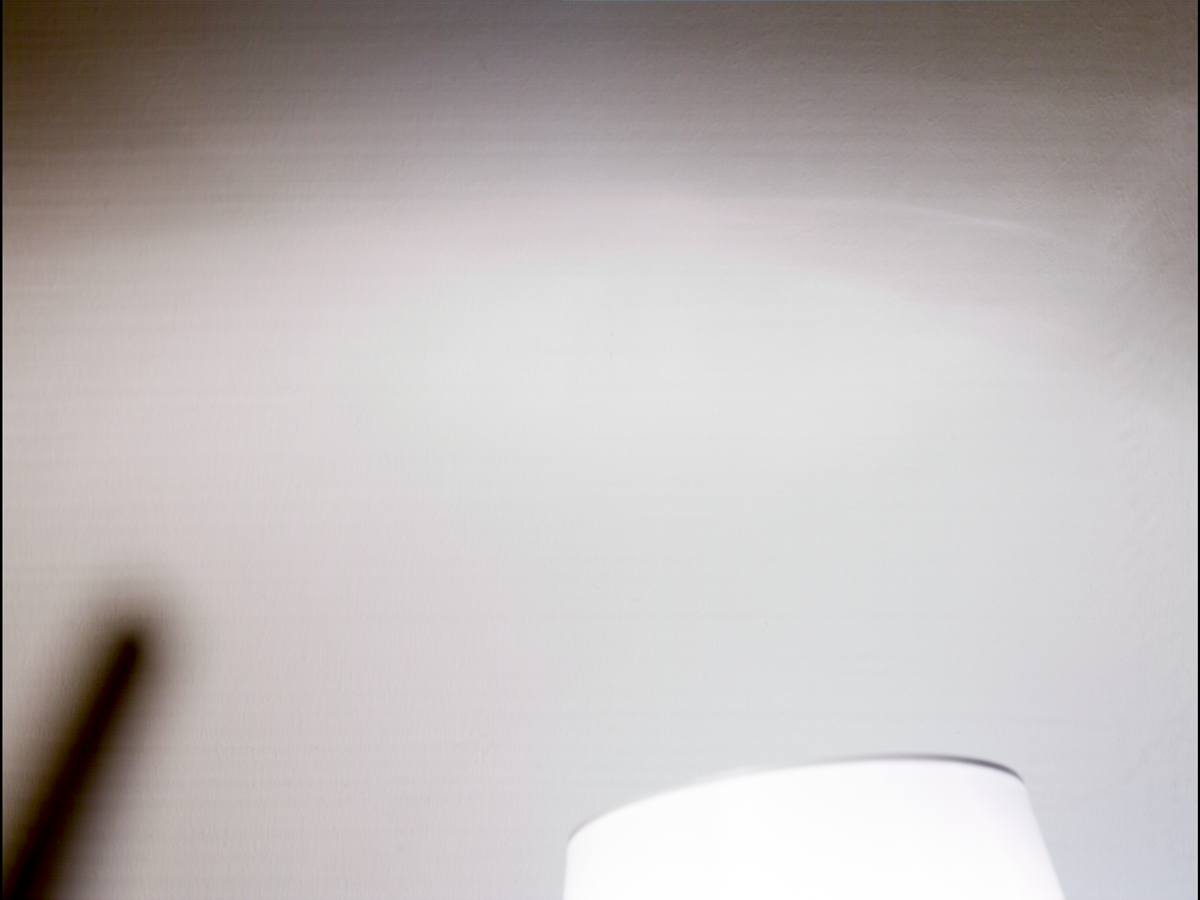
\includegraphics[height=7cm]{images/Vertical-streaks}
\end{center}

These are the result of using the dust cleaning solution on the sensor. Likely the streaks are oil based contaminations. Use the red bottle "smear away" and a swap to clean the sensor. 